\section{Internet Voting}\label{sec:internet-voting}
Internet voting, sometimes referred to as \emph{remote electronic voting}, is a
system of voting where voters are able to cast their votes over the Internet.

% \subsection{Procedure}
% \todo{
%   This doesn't need to be a subsection, just mention it at the start of the
%   Internet Voting section.
% }
\paragraph{Procedure}
The U.S.\ Vote Foundation describes the typical phases involved in conducting an
Internet based election as follows:\cite{e2e-viv}

\begin{enumerate}
  \item \emph{Setup}, during which election officials gather voter information,
    identify election issues and races, design ballots, etc.

  \item \emph{Distribution}, during which election materials are distributed to
    voters: ballots, credentials, voting instructions, etc.

  \item \emph{Voting}, during which voters mark their ballots.

  \item \emph{Casting}, where voters finalize and submit their ballots and
    election officials receive said ballots.

  \item \emph{Tallying}, where election officials count votes, tabulate results,
    and announce winners.

  \item \emph{Auditing}, where (as necessary) vote results are evaluated for
    incorrect results.
\end{enumerate}
% \todo{cite: The Future of Voting — Chapter 3.1}
% cite: The Future of Voting - Chapter 3.1

% \subsection{Requirements}
\paragraph{Requirements}
The requirements for an Internet-based voting system are the same as those for
any other voting system; it must be \emph{secure}, \emph{correct}, and
\emph{private}.
% \todo{Complete section.}

\subsection{Survey of Internet Voting Systems}

In September of 2011 the \emph{Election Assistance Commission (EAC)} published
\emph{``A Survey of Internet Voting,''} which offered a broad review of various
Internet voting systems used between the years of 2000 and
2011.\cite{internet-voting-survey} In total, the survey reviews 30 Internet
voting systems used for elections and primaries, by various parties and
governments, at various levels of government: national, state, and local.

% The survey defines internet voting as,
%
% \begin{displayquote}
%   any system where the voter's ballot selections are transmitted over the
%   Internet from a location other than a polling place to the entity conducting
%   the election.
% \end{displayquote}

% cite: A Survey of Internet Voting Systems - EAC
% https://www.eac.gov/sites/default/files/eac_assets/1/28/SIV-FINAL.pdf

% \begin{description}[style=multiline,font=\normalfont,leftmargin=2cm]
%   \item[2000] Alaska sponsored by the Democratic National Party,
%   \item[2000] Arizona 2000 by the Arizona Democratic Party, and
%   \item[2000] VOI by the FVAP,
%
%   \item[2004] Michigan by the Michigan Democratic Party,
%   \item[2004] SERVE by the FVAP,
%
%   \item[2005/2007/2009/2011] Estonia,
%
%   \item[2008] Democrats Abroad by Democrats Abroad,
%   \item[2008/2010] Arizona 2008/2010 by Arizona Secretary of State's Office,
%   \item[2008] ODBP by Okaloosa County Supervisor of Elections,
%
%   \item[2009] Honolulu by the City of Honolulu,
%
%   \item[2010] District of Columbia by the DC Board of Elections and Ethics,
%   \item[2010] Oregon by the Independent Party of Oregon,
%   \item[2010] West Virginia by the West Virginia Secretary of State,
% \end{description}

\subsubsection{Voting Over the Internet (VOI) --- 2000}

% \subparagraph{Background}
In 1986, the \emph{Uniformed and Overseas Citizens Absentee Voting Act (UOCAVA)}
was passed to render services to merchant marines, uniformed services, and other
overseas civilians. Broadly, UOCAVA mandates that overseas and military
voters be able to remotely register and vote in federal elections, and
designates the Secretary of Defense as the executive agent responsible for
implementing its provisions. Thus, under the \emph{Department of Defense
(DoD)}, the \emph{Federal Voting Assistance Program (FVAP)} was established  to
provide voter assistance, tools, and education to overseas voters with the goal
of enabling overseas voters to vote from anywhere in the world. In pursuit of
this goal, FVAP established procedures for delivering election materials through
domestic, military, and foreign postal systems.

% \paragraph{Objectives and Motivations}
In an effort to eliminate some of the weaknesses inherit in postal systems,
primarily transit times and unreliable delivery guarantees, FVAP established the
\emph{Voting Over the Internet (VOI)} project.

\begin{displayquote}
  ``The pilot project was designed to examine the feasibility of using the
  Internet for remote registration and voting in an effort to overcome the time
  and distance barriers faced by UOCAVA voters. `This was the first time that
  binding votes were cast over the Internet for federal, state, and local
  offices, including the President and Members of
  Congress.'{}''\cite{internet-voting-survey,voi-assessment-report}
\end{displayquote}
% cite: A Survey of Internet Voting Systems - EAC

% \paragraph{Architecture}
The VOI architecture consisted of 3 major components, as illustrated in
Figure~\ref{fig:voi-architecture}:

\begin{itemize}
  \item Citizen infrastructure: any workstation or personal computer with
    Internet access that was available to the voter.

  \item FVAP infrastructure: VOI systems maintained by FVAP, namely the FVAP
    server, which hosted the server-side VOI software, various intrusion
    detection systems, networking infrastructure, and administrative
    workstations.

  \item Local Election Official (LEO) infrastructure: systems managed by
    LEOs, namely servers running VOI software and workstations to interact with
    said software.
\end{itemize}

\begin{figure}[H]
    \centering
    \includegraphics[width=\textwidth]{03-literature/figures/internet-voting/voi/voip}
    % \includesvg[width=\textwidth]{03-literature/figures/internet-voting/voi/voi.svg}
    % \input{03-literature/figures/internet-voting/voi/voi2.pdf_tex}
    % 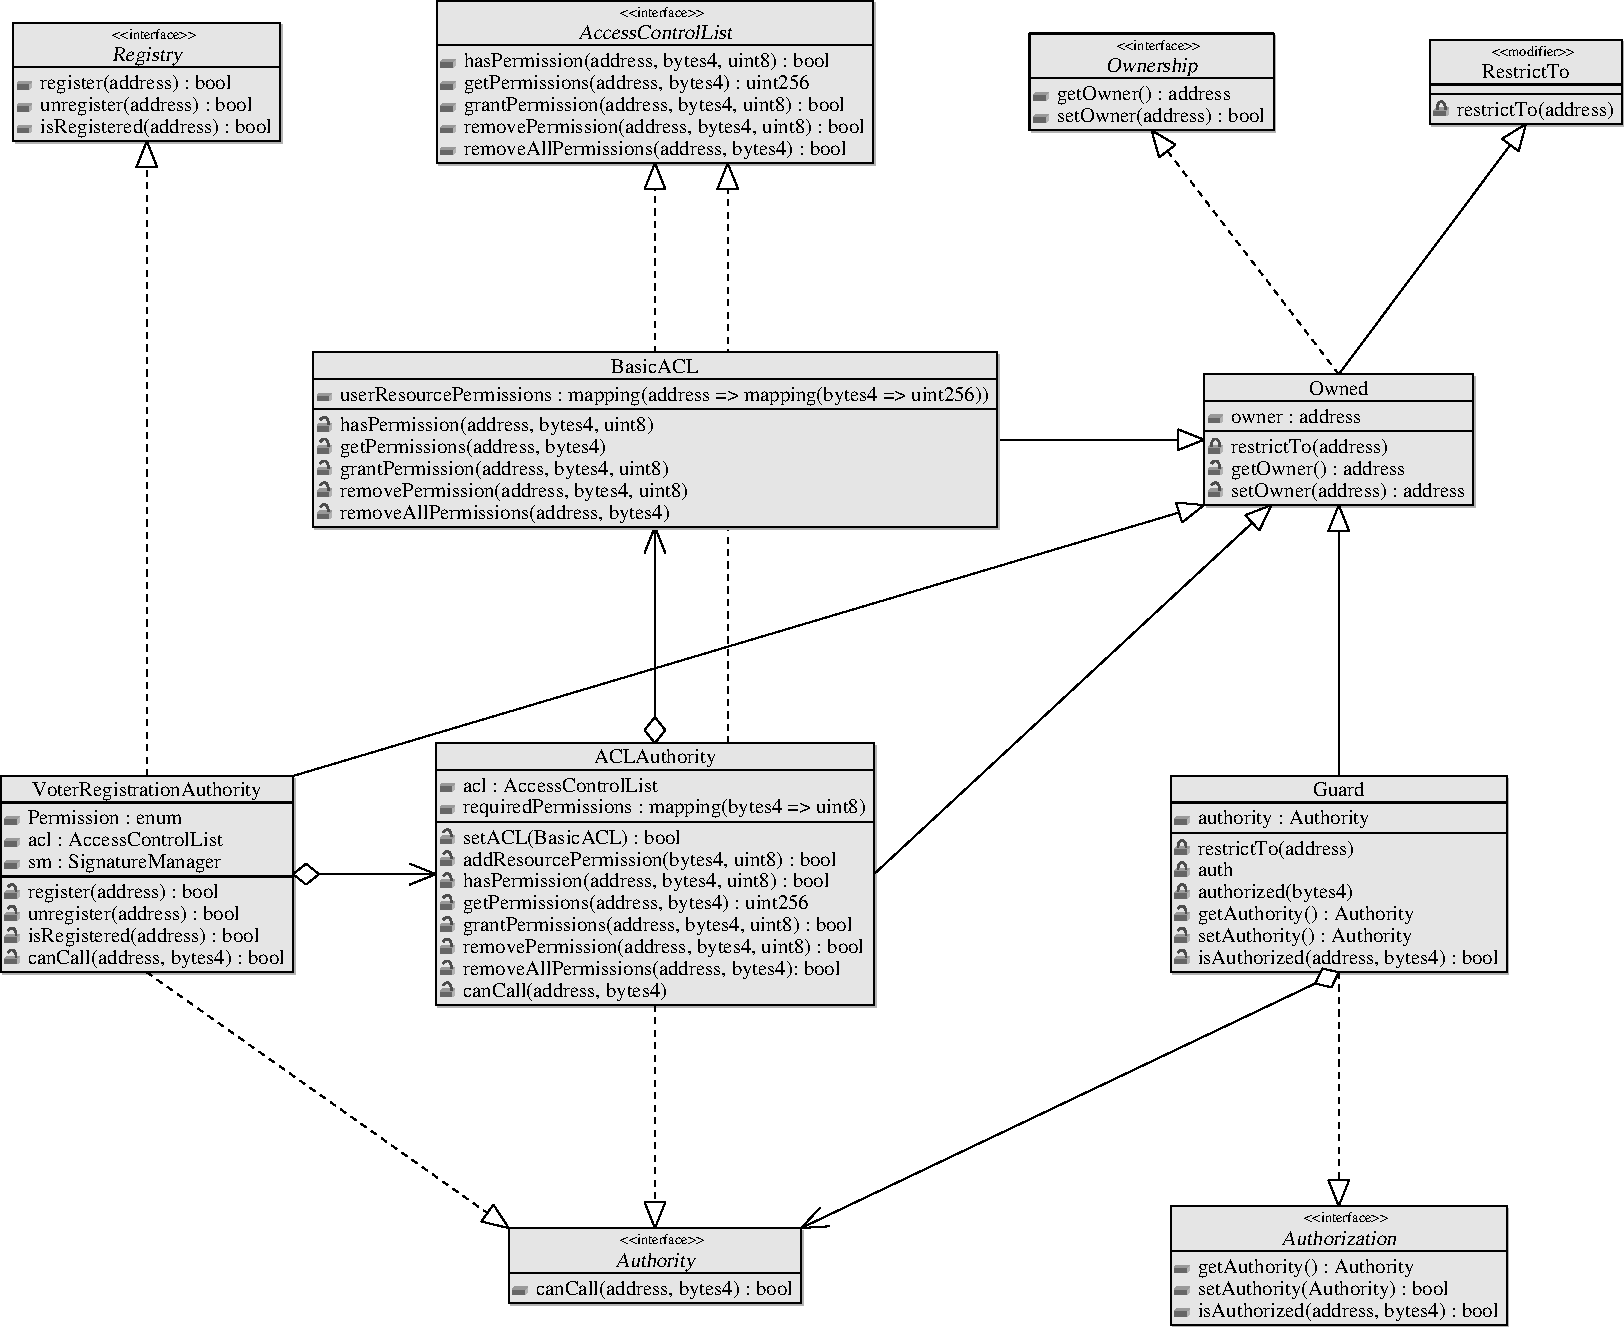
\includegraphics[width=\textwidth]{figures/authorization/figure}
    % \includestandalone[width=\textwidth]{\fig{authorization}}
    \caption{VOI System Architecture~\cite{voi-assessment-report}}\label{fig:voi-architecture}% \label{fig:authorization}
\end{figure}
% cite: Department of Defense Washington Headquarters Services Federal Voting
% cite: https://www.fvap.gov/uploads/FVAP/Reports/voi.pdf
% Assistance Program Voting Over the Internet Pilot Project Assessment Report

\subparagraph{Citizen Infrastructure}
FVAP mailed a CD-ROM to participants containing VOI software, this came in the
form of a Netscape Navigator browser plug-in which provided a graphical user
interface to cast ballots and communicate with the VOI server-side components.
% cite: https://www.fvap.gov/uploads/FVAP/Reports/voi.pdf

% \begin{displayquote}
%   The citizen workstation was the computing platform used by participating
%   citizens to access the Pilot System from their residences or workplaces. The
%   performance requirements for the workstations were intentionally modest to
%   ensure that most existing personal computers would be compatible. The
%   minimum requirements were that the citizen workstation run a Microsoft
%   Windows 95/98 operating system, have a connection to the Internet, and have
%   the Netscape Navigator browser (Version 4.05 or higher, with strong
%   encryption) installed to provide a graphical user interface to the VOI
%   System. Macintosh or UNIX platforms could not be used, nor could Microsoft's
%   Internet Explorer browser. Custom software to enable VOI-specific
%   functionality, in the form of a browser plug-in, was included on a CD-ROM
%   sent to each citizen by the FVAP\@. The CD-ROM also included the strong
%   encryption (128 bit) version of Netscape Navigator for those citizens who
%   needed to upgrade their browser software to be compatible.
% \end{displayquote}

\subparagraph{FVAP Infrastructure}
The FVAP infrastructure consisted of the FVAP server hosting the VOI software,
various networking and power redundancy components to support the server, two
network intrusion detection systems, a server hosting software for creating
electronic ballots, and an administrative workstation for interacting with the
FVAP server. The collective functionalities which this infrastructure provided
included voter authentication, ballot routing to LEO infrastructure, and ballot
creation.

% \begin{displayquote}
% The FVAP server segment was the central component of the VOI System, providing
% the link between the citizen workstations and the LEO servers. The FVAP server
% segment included several different computing platforms, network communication
% components (router, hub), and other components, including a printer, an
% uninterruptible power supply, and a modem for paging system operations and
% maintenance staff. The FVAP segment included the FVAP server, two intrusion
% detection systems, the E-Ballot Tool server, and the FVAP administrative
% workstation.The administrative workstation is a personal computer running a
% Netscape Navigator browser client and is the principal interface to the FVAP
% server for system performance monitoring activities. The two intrusion
% detection system components were positioned on the outside and inside of the
% filtering router to monitor network activities and identify suspicious
% behavior. The intrusion detection system located outside the router is not
% depicted in the system architecture diagram. These two components, along with
% the filtering router and configuration changes to the FVAP server's Microsoft
% Windows NT™ operating system all combined to make the FVAP segment an
% important security barrier protecting the Pilot System.
%
% \emph{FVAP Server}
% The FVAP server included a highly reliable computer hardware server, its
% operating system,database management software, application server software,
% and the VOI custom-developed software. From a functional perspective, the FVAP
% server identified and authenticated users, allowed users to transfer
% Electronic Federal Post Card Applications (EFPCAs) and E-Ballots to and from
% the LEO servers, and performed ``postmarking'' functions. The content of all
% transactions passed through the FVAP server in encrypted form so only the
% addressing information could be read for communications routing purposes.
%
% \emph{E-Ballot Tool Server}
% The E-Ballot Tool server was located within the FVAP server segment security
% architecture and access to it was restricted to specified LEO staff via an
% access control list. This server was dedicated to hosting the E-Ballot Tool
% software. The LEOs used this software to build their electronic ballots. After
% all the component files for the ballots were defined, the LEO would copy those
% associated with a specific ballot style to a floppy disk and upload them to
% the LEO server. No ballots were stored on the E-Ballot Tool server.
% \end{displayquote}

\subparagraph{Local Election Official Infrastructure}
Each LEO site managed a server running VOI software which connected over the
Internet with the FVAP-maintained VOI server and a workstation which allowed
LEOs to perform administrative operations with the server.

% \begin{displayquote}
% Each LEO site had a server that provided connectivity only from the FVAP server
% via the Internet to transmit or receive EFPCAs, E-Ballots, and status messages.
% Each LEO segment included the server hardware platform, the Microsoft Windows NT
% operating system, the VOI custom software, a printer, a removable storage media
% unit, uninterruptible power supply, and network communications devices. Like the
% FVAP segment, each LEO segment had an additional workstation for administration
% of the LEO server.
% \end{displayquote}

% \paragraph{Outcome}
The VOI pilot successfully served 84 volunteers across 4 states. Administrators
did not detect any intrusions into the system during its operation. However, the
DoD acknowledged in their assessment report that one of the major shortcomings
of the pilot was its small sample size, and, that the incentive to attack such a
system would increase as the number of participants
increased.\cite{voi-assessment-report} A future security panel criticized the
VOI system for taking the position that, ``the citizen's workstation is outside
the security perimeter of the system,'' noting that it effectively ignores some
of the most serious kinds of attacks which the system is vulnerable
to.\cite{serve-analysis} On the topic of remote internet voting the DoD
assessment report expressed the following:

\begin{displayquote}[][]
  ``[remote internet voting] is subject to the same security concerns as the
  current VOI System. For this reason, we cannot recommend this alternative as
  an immediate follow-on development to the VOI
  Pilot.\cite{voi-assessment-report}''
\end{displayquote}

%%
% Secure Electronic Registration and Voting Experiment (SERVE) — 2004
%%

\subsubsection{Secure Electronic Registration and Voting Experiment (SERVE) --- 2004}

% In 2002, as directed by Congress and as an immediate follow-on development to
% the VOI pilot, the DoD began work on a remote Internet voting project.

% \subparagraph{Background}
In 2002, following the VOI project, Congress instructed the DoD to carry out a
larger demonstration project, ``under which absent uniformed services voters are
permitted to cast ballots in the regularly scheduled general election for
Federal office.''\cite{serve-bill} To fulfill this mandate FVAP contracted
Accenture to build \emph{The Secure Electronic Registration and Voting
Experiment} (SERVE).

% \paragraph{Objectives and Motivations}
SERVE was built under the United States' Department of Defense's (DoD) Federal
Voting Assistance Program (FVAP) to be deployed for the 2002 or 2004 elections.
Broadly, the motivations behind SERVE were to produce an Internet-based voting
system to reduced barriers to voting for Americans living overseas; specifically
the objectives of the project were to:

\begin{enumerate}
  \item ``assess whether the use of electronic voting technology could improve the
    voting participation success rate for UOCAVA
    citizens,''\cite{dod-expanding-electronic-voting} and

  \item ``assess the potential impact on state and local election administration
    of an automated alternative to the conventional by-mail process of absentee
    registration and voting.''\cite{dod-expanding-electronic-voting}
\end{enumerate}

Fifty counties covering 7 states were targeted for participation and the system was
designed to handle both the registration and voting process.

\paragraph{Architecture}
SERVE shared many architectural-similarities to VOI which are reflected in the
SERVE architecture diagram seen in Figure~\ref{fig:serve-architecture}\@:

\begin{itemize}
  \item SERVE was designed as a web-based service which a voter could connect to
    via web browser.

  \item LEOs managed a local server which could be used to interact with
    the central SERVE system.

  \item The central SERVE system, which performed the bulk of the system
    processing, was maintained by FVAP and stored voter information until the
    appropriate LEO server downloaded it.
\end{itemize}
% to be stored by the central SERVE system that was to be maintained by FVAP\@.

The system was described as consisting of eight integrated subsystems:
Identification and Authentication; Common Services; Voter Registration; Election
Administration; Ballot Definition; Voting; Download and Decryption; and
Tabulation.

\begin{figure}[H]
    \centering
    \includegraphics[width=\textwidth]{03-literature/figures/internet-voting/serve/architecture}
    \caption{SERVE System Architecture~\cite{internet-voting-survey}}\label{fig:serve-architecture}% \label{fig:authorization}
\end{figure}

%  would
% handle identification, registration, authentication, and ballot casting
% procedures. Ballots would be encrypted with LEO  which allowed them to access voter data and encrypted ballots which were

To participate one had to have a military ID (a Common Access Card), or could
enroll in the SERVE system by presenting face-to-face proof of citizenship to a
SERVE official. Once enrolled and registered, a participant could vote via a web
browser through the SERVE site. Figure~\ref{fig:serve-voting-protocol} outlines
the protocol used for casting a ballot through the SERVE web application.

\begin{figure}[H]
    \centering
    \includegraphics[width=0.8\textwidth]{03-literature/figures/internet-voting/serve/protocol}
    \caption{SERVE Voting Protocol~\cite{internet-voting-survey}}\label{fig:serve-voting-protocol}% \label{fig:authorization}
\end{figure}

% \paragraph{Outcome}
SERVE received harsh criticism from independent system reviewers, members of the
\emph{Security Peer Review Group (SPRG)}, academics and industry professionals
who were assembled by FVAP to evaluate the system. A group of these members
independently publicized concerns regarding the security of the system and
Internet-based voting systems more broadly.\cite{serve-analysis}

% \subparagraph{Vulnerabilities}
The report published notes that SERVE suffers from a number of vulnerabilities
and goes into great detail regarding the risks these vulnerabilities pose and
the complexity of performing various attacks to take advantage of these
vulnerabilities. The report noted:\cite{serve-analysis}

\begin{enumerate}
  \item Lack of voter-verified audit trails and vulnerabilities to insider
    attacks. Vulnerabilities in software are difficult to find and intentionally
    obfuscated vulnerabilities are even more so. The essentially unauditable
    nature of electronic voting systems necessitate some form of voter-verified
    audit trail.

  \item Privacy. Several system design issues were identified which would allow
    LEOs or SERVE administrators to tie a ballot to a voter's identity.

  \item Vote Buying/Selling. The nature of Internet voting makes selling
    credentials for voting systems a very real possibility.

  \item Intimidation. Voter intimidation is a problem which all remote voting
    systems must contend with, this problem extends to Internet voting systems.

  \item Large-Scale Impact. Electronic voting machines, if compromised, might
    enable attackers to modify or damage tens or hundreds of thousands of
    ballots. Internet voting systems face this same issue, except on a much
    larger scale; the entire system essentially acts as a single electronic
    voting machine, significantly increasing the scale of impact if compromised.
    Paper-based systems do not face these same exposures.

  \item Too Many Potential Attacks. Electronic systems present a large attack
    surface, exposure to the Internet presents even more. Mitigation of all of
    the kinds of attacks possible would not be feasibility.

  \item Many Sources of Attacks. Elections held over the Internet are vulnerable
    to attacks from around the globe; nation-state entities, terrorists,
    individual hackers and more would all have the ability to attack system.

  \item Undetectable Attacks. Electronic systems make detecting attacks
    extremely difficult and the lack of a detected attack on a system does not
    prove that no attack occurred.

  \item On-screen Electioneering. Many states prevent campaigning within some
    distance of a polling place; however, no such laws exist to prevent ISPs,
    web browsers, or other entities from displaying ads to voters.
\end{enumerate}

% The details of the vulnerabilities reported
% are discussed in further detail in Section~\ref{section:shared-weaknesses},
% however, the report notes:

In addition the report had this to say about future attempts at building
Internet voting systems:

\begin{displayquote}
  ``Like the proponents of SERVE, we believe that there should be better support
  for voting for our military overseas. Still, we regret that we are forced to
  conclude that the best course is not to field the SERVE system at all. Because
  the danger of successful, large-scale attacks is so great, we reluctantly
  recommend shutting down the development of SERVE immediately and not
  attempting anything like it in the future until both the Internet and the
  world's home computer infrastructure have been fundamentally redesigned, or
  some other unforeseen security breakthroughs appear.''\cite{serve-analysis}
\end{displayquote}

In response to these criticisms and concerns documented in this report, the
then-Deputy Secretary of Defense Paul Wolfowitz decided that the SERVE project
would not go forward as planned for the 2004 election, effectively killing the
project.\cite{dod-expanding-electronic-voting} Three years later the DoD
published a report which downplayed the criticisms and concerns published by the
SPRG members.\cite{dod-expanding-electronic-voting} In reaction to this DoD
report, the members of the SPRG independently publicized a response which
criticized the report for downplaying the concerns laid out in their initial
security analysis of SERVE, and further reiterated their concerns regarding
Internet voting. The members of the SPRG noted again that the issues faced by
SERVE are ones which are not capable of being fixed by a better design or
architecture of Internet voting systems, because the fundamental issues are ones
which could only be fixed by redesigning both the Internet and personal
computers.\cite{comment-on-dod-report}

% \subsubsection{Integrated Voting Alternative Site (IVAS)}
% September 2006

% Interim Voting Assistance System
% https://graphics8.nytimes.com/packages/pdf/national/2006_IVAS_report.pdf

% Integrated Voting Alternative Site
% https://www.fvap.gov/uploads/FVAP/Reports/ivas06.pdf
% \todo{What does IVAS stand for? A: It stands for both.}
% \todo{Complete section.}

\subsubsection{D.C. Digital Vote-by-Mail System (DVBM) --- 2010}

% \subparagraph{Background}
In 2009 the \emph{Military and Overseas Voter Empowerment Act (MOVE)} was
passed. This act amended UOCAVA and other statutes to provide further protections
to eligible citizens. Specifically the act aimed to reduce the number of ballots
which are not counted due to late receipt. MOVE accomplishes this by requiring
that states send absentee ballots no later that 45 days prior to election day.
MOVE goes further by requiring that all registration material and blank ballots
be available electronically and removes requirements regarding notarization on
voting applications and ballots.\cite{MOVE}

% \begin{displayquote}
%   In 2010, Washington, D.C.\ developed an Internet voting pilot project that was
%   intended to allow overseas absentee voters to cast their ballots using a
%   website.
%   % https://jhalderm.com/pub/papers/dcvoting-fc12.pdf
% \end{displayquote}

% \paragraph{Objectives and Motivations}
In search of a solution to improve their compliance with the MOVE act,
Washington's District of Columbia Board of Elections and Ethics (DCBOEE/BOEE)
planned to launch an Internet voting system, the D.C. Digital Vote-by-Mail
(DVBM) system, for use in the November 2010 general election. The project was
developed in partnership with the Open Source Digital Voting (OSDV) Foundation's
TrustTheVote project, who viewed the project as a mostly academic
effort.\cite{trust-the-vote-dc-pilot} The system was slated to be operational in
time for the November 2010 general election and aimed to provide two primary
functionalities:\cite{internet-voting-survey,dc-voting-system}
\begin{enumerate}
  \item allow voters to electronically access voting materials
  \item allow voters to optionally cast their ballot over the internet
\end{enumerate}

% \paragraph{Architecture}
The DVBM architecture, illustrated in Figure~\ref{fig:dvbm-architecture}, was
developed as a web application using the Ruby on Rails framework; was hosted
using the Apache web server; used MySQL as its database technology, which stored
the global election state (voters' names, addresses, etc.); and used the
underlying (Linux) filesystem to store encrypted ballots cast by voters. When
the voting phase of the election was complete, election officials would transfer
the encrypted ballots to an air-gapped computer for decryption and printing.
Printed ballots would be counted alongside other mail-in absentee
ballots.\cite{dc-voting-system}

\begin{figure}[H]
    \centering
    \includegraphics[width=\textwidth]{03-literature/figures/internet-voting/dc/architecture}
    % \includesvg[width=\textwidth]{03-literature/figures/internet-voting/voi/voi.svg}
    % \input{03-literature/figures/internet-voting/voi/voi2.pdf_tex}
    % 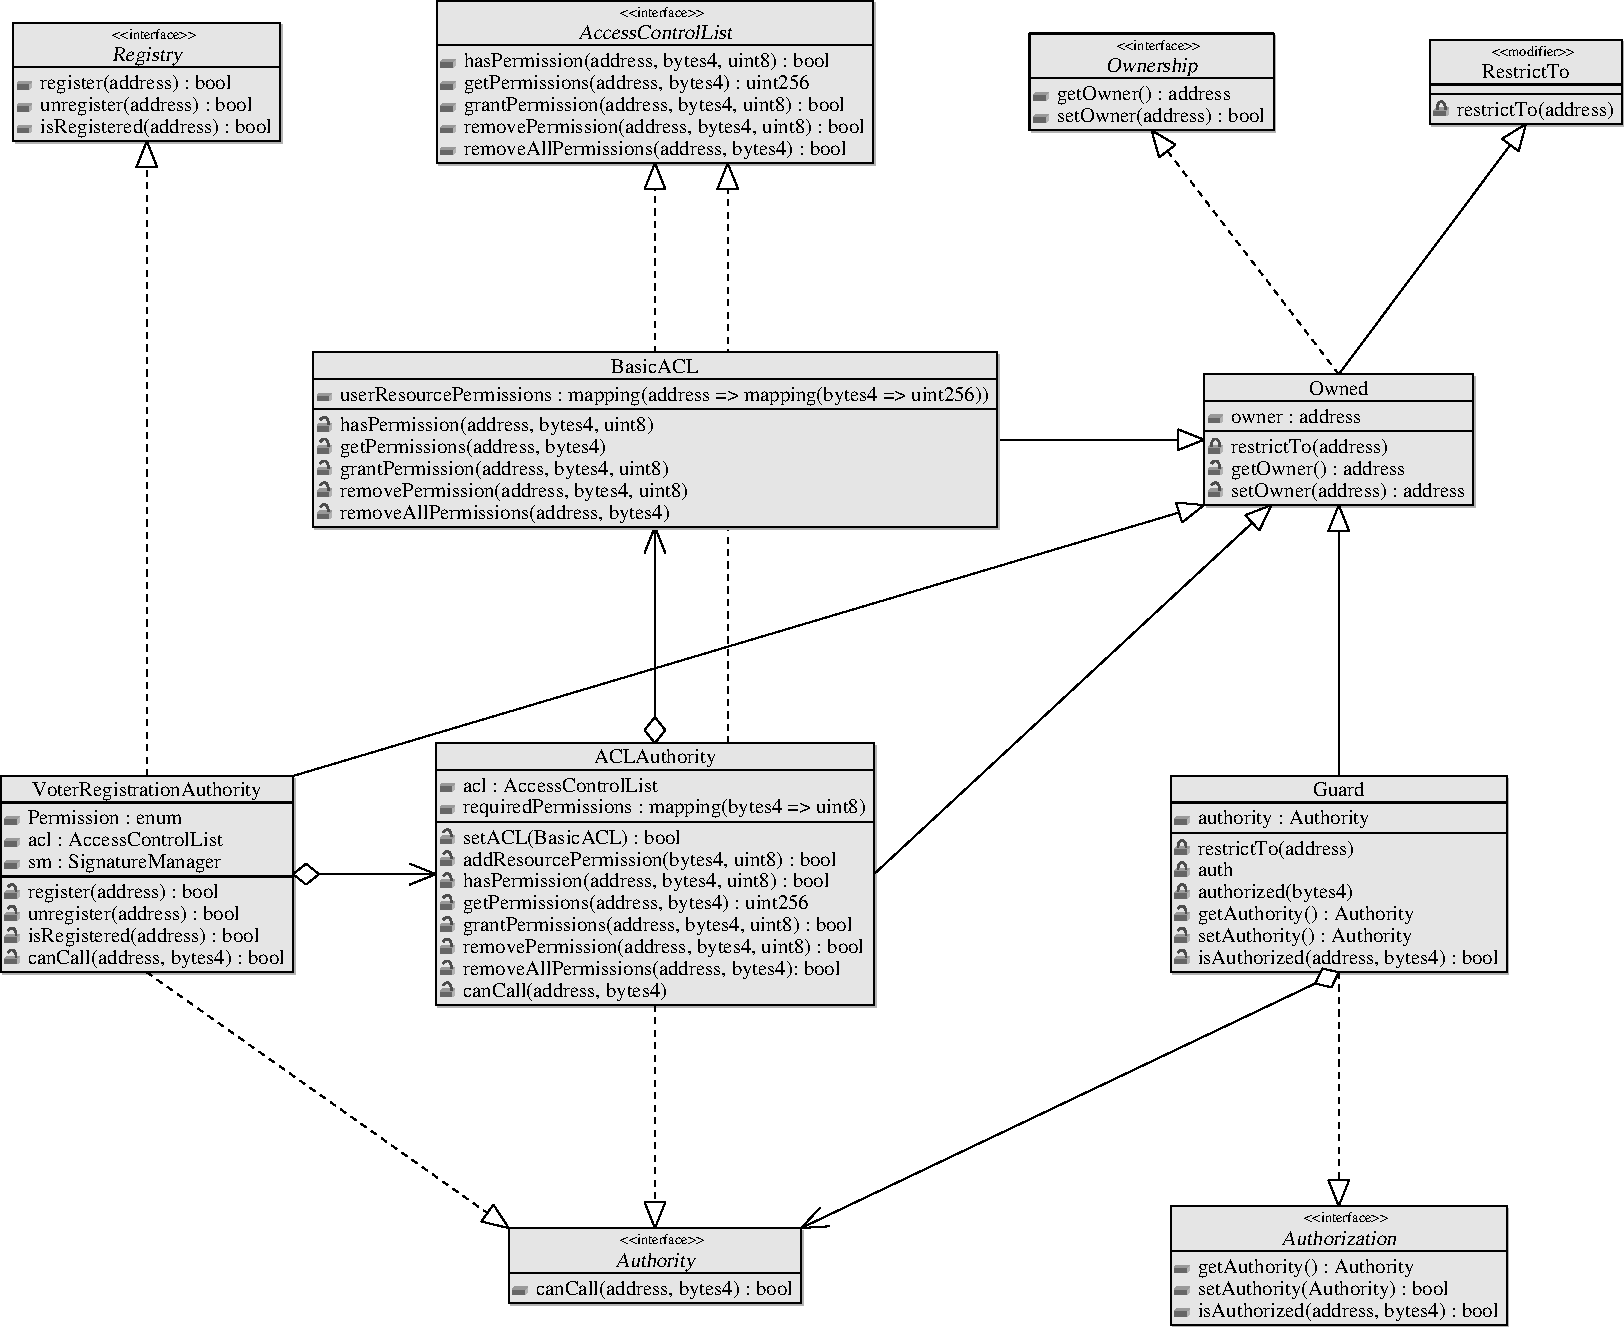
\includegraphics[width=\textwidth]{figures/authorization/figure}
    % \includestandalone[width=\textwidth]{\fig{authorization}}
    \caption{DVBM System Architecture~\cite{dc-voting-system}}\label{fig:dvbm-architecture}% \label{fig:authorization}
\end{figure}

Prior to the official launch of the system the BOEE opted to conduct a mock
election where members of the public, researchers, and hackers alike were
invited to to test the functionality of the system, discover vulnerabilities,
and attempt to compromise the security, reliability, and availability of the
system.\cite{internet-voting-survey,dc-voting-system,trust-the-vote-dc-pilot}

% \paragraph{Outcome}
Within 48 hours of the system going live researchers from The University of
Michigan, playing the role of an attacker, demonstrated a number of
vulnerabilities and attacks on on the system and managed to gained near-complete
control of the election server. Their intrusion was not detected for nearly 2
days.\cite{dc-voting-system}
% Prior to its launch election officials held a mock election to test the security
% of the system, inviting researchers and hackers alike to attempt to compromise
% the security, reliability, and availability of the system. A number of attacks
% were demonstrated and researchers were able to:

Demonstrated vulnerabilities included being able to:
\begin{itemize}
  \item penetrate the network of the election software
  \item determine voter's identities
  \item locate unencrypted ballots, thus mapping voter's identities to their
    personal votes
  \item modify ballots
  \item cast fake ballots
  \item modify the election system software itself
\end{itemize}

Once election officials became aware of the attack, the mock election was
suspended, five days ahead of schedule, citing ``usability issues.'' Election
officials later confirmed that they were unable to detect the attack or network
presence using their intrusion detection system. Due to the test results, the
portion of the system which allowed for ballots to be submitted over the
Internet was not used.\cite{dc-voting-system}

\subsubsection{Estonia --- 2005}
Estonia began using Internet voting in 2005\cite{internet-voting-survey}; in the
2015 Estonian parliamentary elections, 30.5\% of all voters voted over the
Internet. Estonia maintains what is likely the most advanced national
identification cards in the world. Estonian IDs are part of a \emph{Public Key
Infrastructure (PKI)} where IDs serve as smart cards which possess two RSA key
pairs: one for signing and one for authentication; these cryptographic functions
are performed directly on the card. The signatures produced by these IDs are
used extensively throughout the country and are considered legally binding.
These cryptographic IDs allow Estonia to provide voter authentication
capabilities that cannot be reproduced in the US.\ Despite the advanced
authentication capabilities that Estonia is able to achieve, researchers in 2014
devised a number of attacks that could be performed on the Estonian voting
system to spoil ballots, damage ballot secrecy, and steal or drop votes. The
researchers also criticized the transparency and operational security of the
system, noting that videos of the administration processes --- provided for
transparency purposes --- recorded administrators entering root passwords,
revealed network credentials which had been posted on a wall, and showed
administrators using USB drives containing personal files to move sensitive
election materials between systems.\cite{estonia}

% \subsection{Shared Weaknesses}\label{section:shared-weaknesses}
% There are a number of shared weaknesses and vulnerabilities exposed across these
% internet voting systems which the systems incur due to the underlying
% architecture of the systems, their Internet, the personal computer, and remote
% voting.
%
% \begin{enumerate}
%   \item Lack of voter-verified audit trails.
%   \item Vulnerabilities to insider attacks.
%   \item Privacy.
%   \item Vote Buying/Selling.
%   \item Intimidation.
%   \item Large-Scale Impact.
%   \item Too Many Potential Attacks.
%   \item Many Sources of Attacks.
%   \item Undetectable Attacks.
%   \item On-screen Electioneering.
% \end{enumerate}

% \todo{
%   Should I add a shared weaknesses section here and remove some of the
%   demonstrated attacks from the individual systems?
% }
